\documentclass[10pt,conference,compsocconf,a4paper]{IEEEtran}

\usepackage{graphicx}
\usepackage{amsmath, amssymb}
\usepackage{commath}
\usepackage{booktabs}
\usepackage{siunitx}
\usepackage[labelformat=simple, labelfont=normalfont]{subcaption}  % Side-by-side figures
\usepackage[labelfont=sc]{caption}  % Using captionof outside of figure environment
\usepackage[colorlinks, bookmarks=false, citecolor=black, linkcolor=black, urlcolor=blue]{hyperref}  % Cite colors + autoref
\usepackage{xurl}  % hypen breaks in urls

\renewcommand{\vec}[1]{\boldsymbol{#1}}
\newcommand{\vunit}[1]{\ [\si{#1}]}
\newcommand{\nunit}[1]{\ \si{#1}}

% braces around equation number in referencing
\makeatletter
\let\oldtheequation\theequation
\renewcommand\tagform@[1]{\maketag@@@{\ignorespaces#1\unskip\@@italiccorr}}
\renewcommand\theequation{(\oldtheequation)}
\makeatother

% Prevent latex from streching out paragraph spacings
\raggedbottom

% braces around subfig number
\renewcommand\thesubfigure{\,(\alph{subfigure})}

% Smallcaps short autoref
\newcommand*{\shortautoref}[1]{%
	\begingroup
	\def\equationautorefname{\textsc{Eq.}}%
	\def\tableautorefname{\textsc{Tab.}}%
	\def\figureautorefname{\textsc{Fig.}}%
	\autoref{#1}%
	\endgroup
}

% Itemize spacing
\let\olditemize=\itemize
\let\endolditemize=\enditemize
\renewenvironment{itemize}{\olditemize \itemsep0em}{\endolditemize}

% subfigure spacing
\captionsetup[subfigure]{aboveskip=1pt}

\begin{document}
\title{BIO-465 -- Project\\A network model of cortical surround suppression}

\author{
	Etienne Objois, Niels Vadot\\
	\textit{EPFL, Switzerland}
}

\maketitle

\begin{abstract}
	We explore neuronal population models and use them to model cortical surround suppression.
	Cortical surround suppression is a phenomenon where the presence of nearby neighbours causes a neuron to have a lower activity level than if it were alone.
	We also expore the orientation tuning phenomenon, where the surround suppression is more or less strong, depending on the overlap between the external stimulus and the receptive fields.
	The source code is available at \cite{cs456_source}.
\end{abstract}

\section{Rate models of neuronal populations}

	A neuronal population is composed of multiple neurons, which can each be individually modeled. In the simple model from \shortautoref{eq:model_neuron}, a neuron is described by the voltage across its membrane $h(t)$, resistivity $R$ to input currents $I(t) = I_{\text{ext}}(t) + I_{\text{network}}(t)$, a relaxation time constant $\tau$, and an activity level $A(t)$ defined in terms of a filter $\alpha(s)$ and gain function $F(h)$ in the equation $A(t) = \int_0^\infty \alpha(s) F(h(t-s)) \dif{s}$.

	\begin{equation} \label{eq:model_neuron}
		\tau \dot h(t) = -h(t) + R I(t)
	\end{equation}

	In a population, every neuron is modeled individually according to \shortautoref{eq:model_neuron}, and attributed an index $k$. We furthermore model the network currents linearly as in \shortautoref{eq:model_current}, by introducing a weight parameter $W_{kn}$, which describes the influence of neuron $n$ on neuron $k$.

	\begin{equation} \label{eq:model_current}
		I_{\text{network},k}(t) = \sum_n W_{kn} A_n(t)
	\end{equation}

	A further simplification can be made by letting $\alpha(s)$ be a very sharp filter, approximatively a Dirac delta. Then $A(t) \approx F(h(t))$.

	We can rewrite the entire system as one equation in matrix form, where $\vec h = (h_1, \cdots, h_n)$, $\vec R = (R_1, \cdots, R_n)$, etc., and $\odot$ is the elementwise product :

	\begin{equation} \label{eq:model_population}
		\vec{\tau} \odot \dot{\vec h} = -\vec h + \vec R \odot (\mathsf W \vec F(\vec h)) + \vec R \odot \vec{I_{\text{ext}}}
	\end{equation}

	\shortautoref{eq:model_population} models a population of neurons, but can also be interpreted to model an ensemble of populations. This is assumed from now on, and a more detailed proof and renormalization is given in \shortautoref{sec23}.

\section{Fixed vs. recurrent inhibition}
\label{sec1}

	\subsection{Excitatory population with self-coupling}
	\label{sec11}

		We model a single population according to \shortautoref{eq:model_population}, and assume constant input current $I_{\text{ext}}$. The gain function is defined as $F(h) = \frac 12 (1 + \mathrm{tanh}(h))$.
		
		The self-coupling appears in the diagonal terms of $\mathsf W$, and in this case there is only self-coupling, since $\mathsf W$ reduces to a scalar.

		We vary the constant input current in \shortautoref{figure:pop_single_nonlin} and study $t < 7$ (before the delta spike). The simulation is started at $h(0) \neq 0$ in order to break symmetry of the gain function. For all currents, the activity levels out over time. We can observe three regimes.
		(1) At $I_{\text{ext}} \lesssim -1 \nunit{\ampere}$, there is too much negative current (i.e. too many negative charges arrive too fast, which depolarizes the population) and the self-coupling is not enough to maintain activity levels, which decay to nearly zero.
		(2) At $I_{\text{ext}} \gtrsim -1 \nunit{\ampere}$, the opposite happens, and self-coupling manages to drive the activity levels to nearly one.
		(3) At $I_{\text{ext}} \approx -1 \nunit{\ampere}$, the external current and self-coupling nearly cancel out, leaving the activity somewhere between zero and one.

		The introduction of a delta spike at $t = 7$ makes the activity levels jump, which then recover and tend back to the same equilibrium as before the spike. For a same total charge, unsaturated neurons ($0 \lesssim A \lesssim 1$) jump a larger amplitude and take more time to recover than saturated neurons ($A \approx 0$ or $A \approx 1$). The jump is asymetric with respect to charge sign : if $A > \frac 12$, then for $q < 0$ the perturbation is greater than for $q > 0$ (and vice-versa). For total charges of the same sign, the size of the jump is largest for the largest absolute charge.

		\begin{figure}
			\centering
			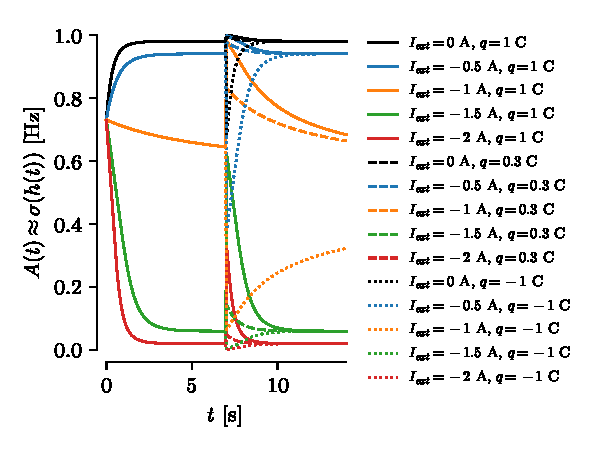
\includegraphics[width=0.5\textwidth]{figures/pop_single_nonlin.pdf}
			\caption{Single population with constant input and a delta spike of total charge $q$ at $t = 7$. Parameters $W = 2$, $\tau = 0.6, R = 1, h(0) = 0.5$.}
			\label{figure:pop_single_nonlin}
		\end{figure}

		In order to get insight into the behavior of the coupling strength, \shortautoref{figure:pop_single_nonlin_phase} shows a 1D phase plot of the differential equation. Fixed points solutions to $\dot h = 0$. $I_{\text{ext}}$ controls the vertical offset of the curves but more interestingly $W$ controls the appearance of two local extrema, and therefore the possibility of two other solutions. This happens when the curvature changes sign, and critically when the derivative is null. Solving $\partial^2_h \dot h = 0$ and $\partial_h \dot h = 0$ for $h$ and $W$, we find $h_{\text{crit}} = 0$ and $W_{\text{crit}} = 2/R$. When $W < W_{\text{crit}}$, only one stable solution exists. When $W > W_{\text{crit}}$, three solutions can exist (two stable, and one unstable at $h = 0$) depending on the value of $I_{ext}$.
		
		If we furthermore impose $\dot h = 0$ at the critical value, then we get $I_{\text{crit}} = -1/R$. When $I < I_{\text{crit}}$, the three solutions can exist (provided the current is not too negative), whereas when $I > I_{\text{crit}}$ only one solution exists.

		Intuitively, the current has to be depolarizing enough but the self-coupling strong enough to compensate, and create a second solution. \shortautoref{figure:pop_single_threesol} demonstrates a set of parameters for which there are two stable solutions, and one unstable solution.

		\begin{figure}
			\centering
			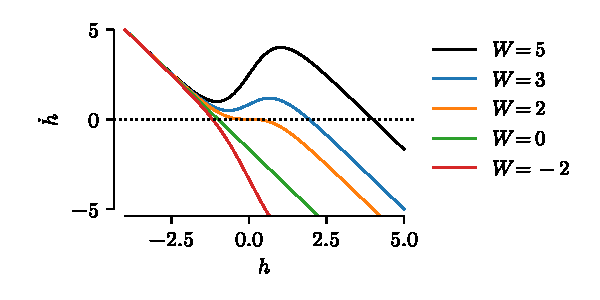
\includegraphics[width=0.5\textwidth]{figures/pop_single_nonlin_phase.pdf}
			\caption{1D phase plot of a single population. Parameters $\tau = 0.6, R = 1, I_{\text{ext}}= -1$. Critical values are $W_{\text{crit}} = 2$ and $I_{\text{crit}} = -1$.}
			\label{figure:pop_single_nonlin_phase}
		\end{figure}

		\begin{figure}
			\centering
			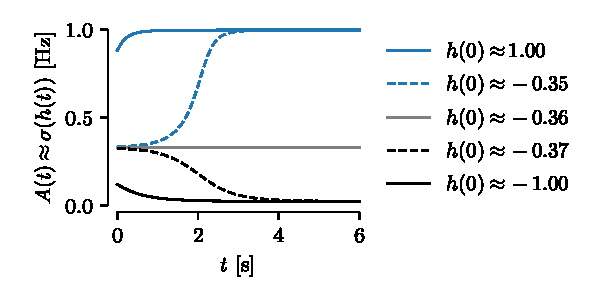
\includegraphics[width=0.5\textwidth]{figures/pop_single_threesol.pdf}
			\caption{Simulation of a single population with three fixed points. Parameters $W = 5, R = 1, I_{\text{ext}} = -2$.}
			\label{figure:pop_single_threesol}
		\end{figure}

	\subsection{Inhibition-stabilized network (ISN)}
	\label{sec12}

\section{Modeling surround suppression}
\label{sec2}

	\subsection{Network mechanisms of surround suppression}
	\label{sec21}

	\subsection{Orientation tuning of surround suppression}
	\label{sec22}

	\subsection{Surround suppression in networks with bio-plausible connectivity}
	\label{sec23}

% \begin{figure}
% 	\caption{Average reward of Q-learning player for every 50 games. $\epsilon = 0.1$}

% 	\includegraphics[width = 0.4\textwidth]{figures/q1.png}
% 	\label{figure:q1}
% \end{figure}

\newpage
\bibliographystyle{IEEEtran}
\bibliography{literature}

% \newpage
% \appendix

% 	moar uwu

\end{document}
